\section[Theorie]{Theorie \textnormal{\cite{faraday}}}
\label{sec:theorie}

\subsection{Bandstruktur}

\begin{figure}
    \centering
    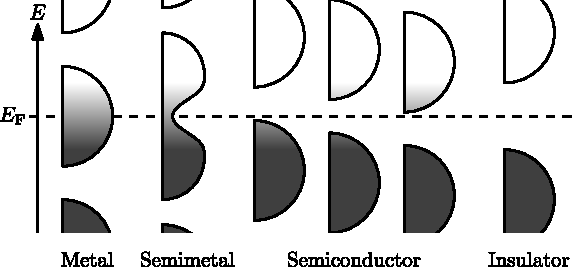
\includegraphics[width=0.8\textwidth]{content/grafik/bandstructure.pdf}
    \caption{Bandstrukturen verschiedener Materialklassen im Vergleich. \cite{wiki_band}}
    \label{fig:baender}
\end{figure}

\begin{figure}
    \centering
    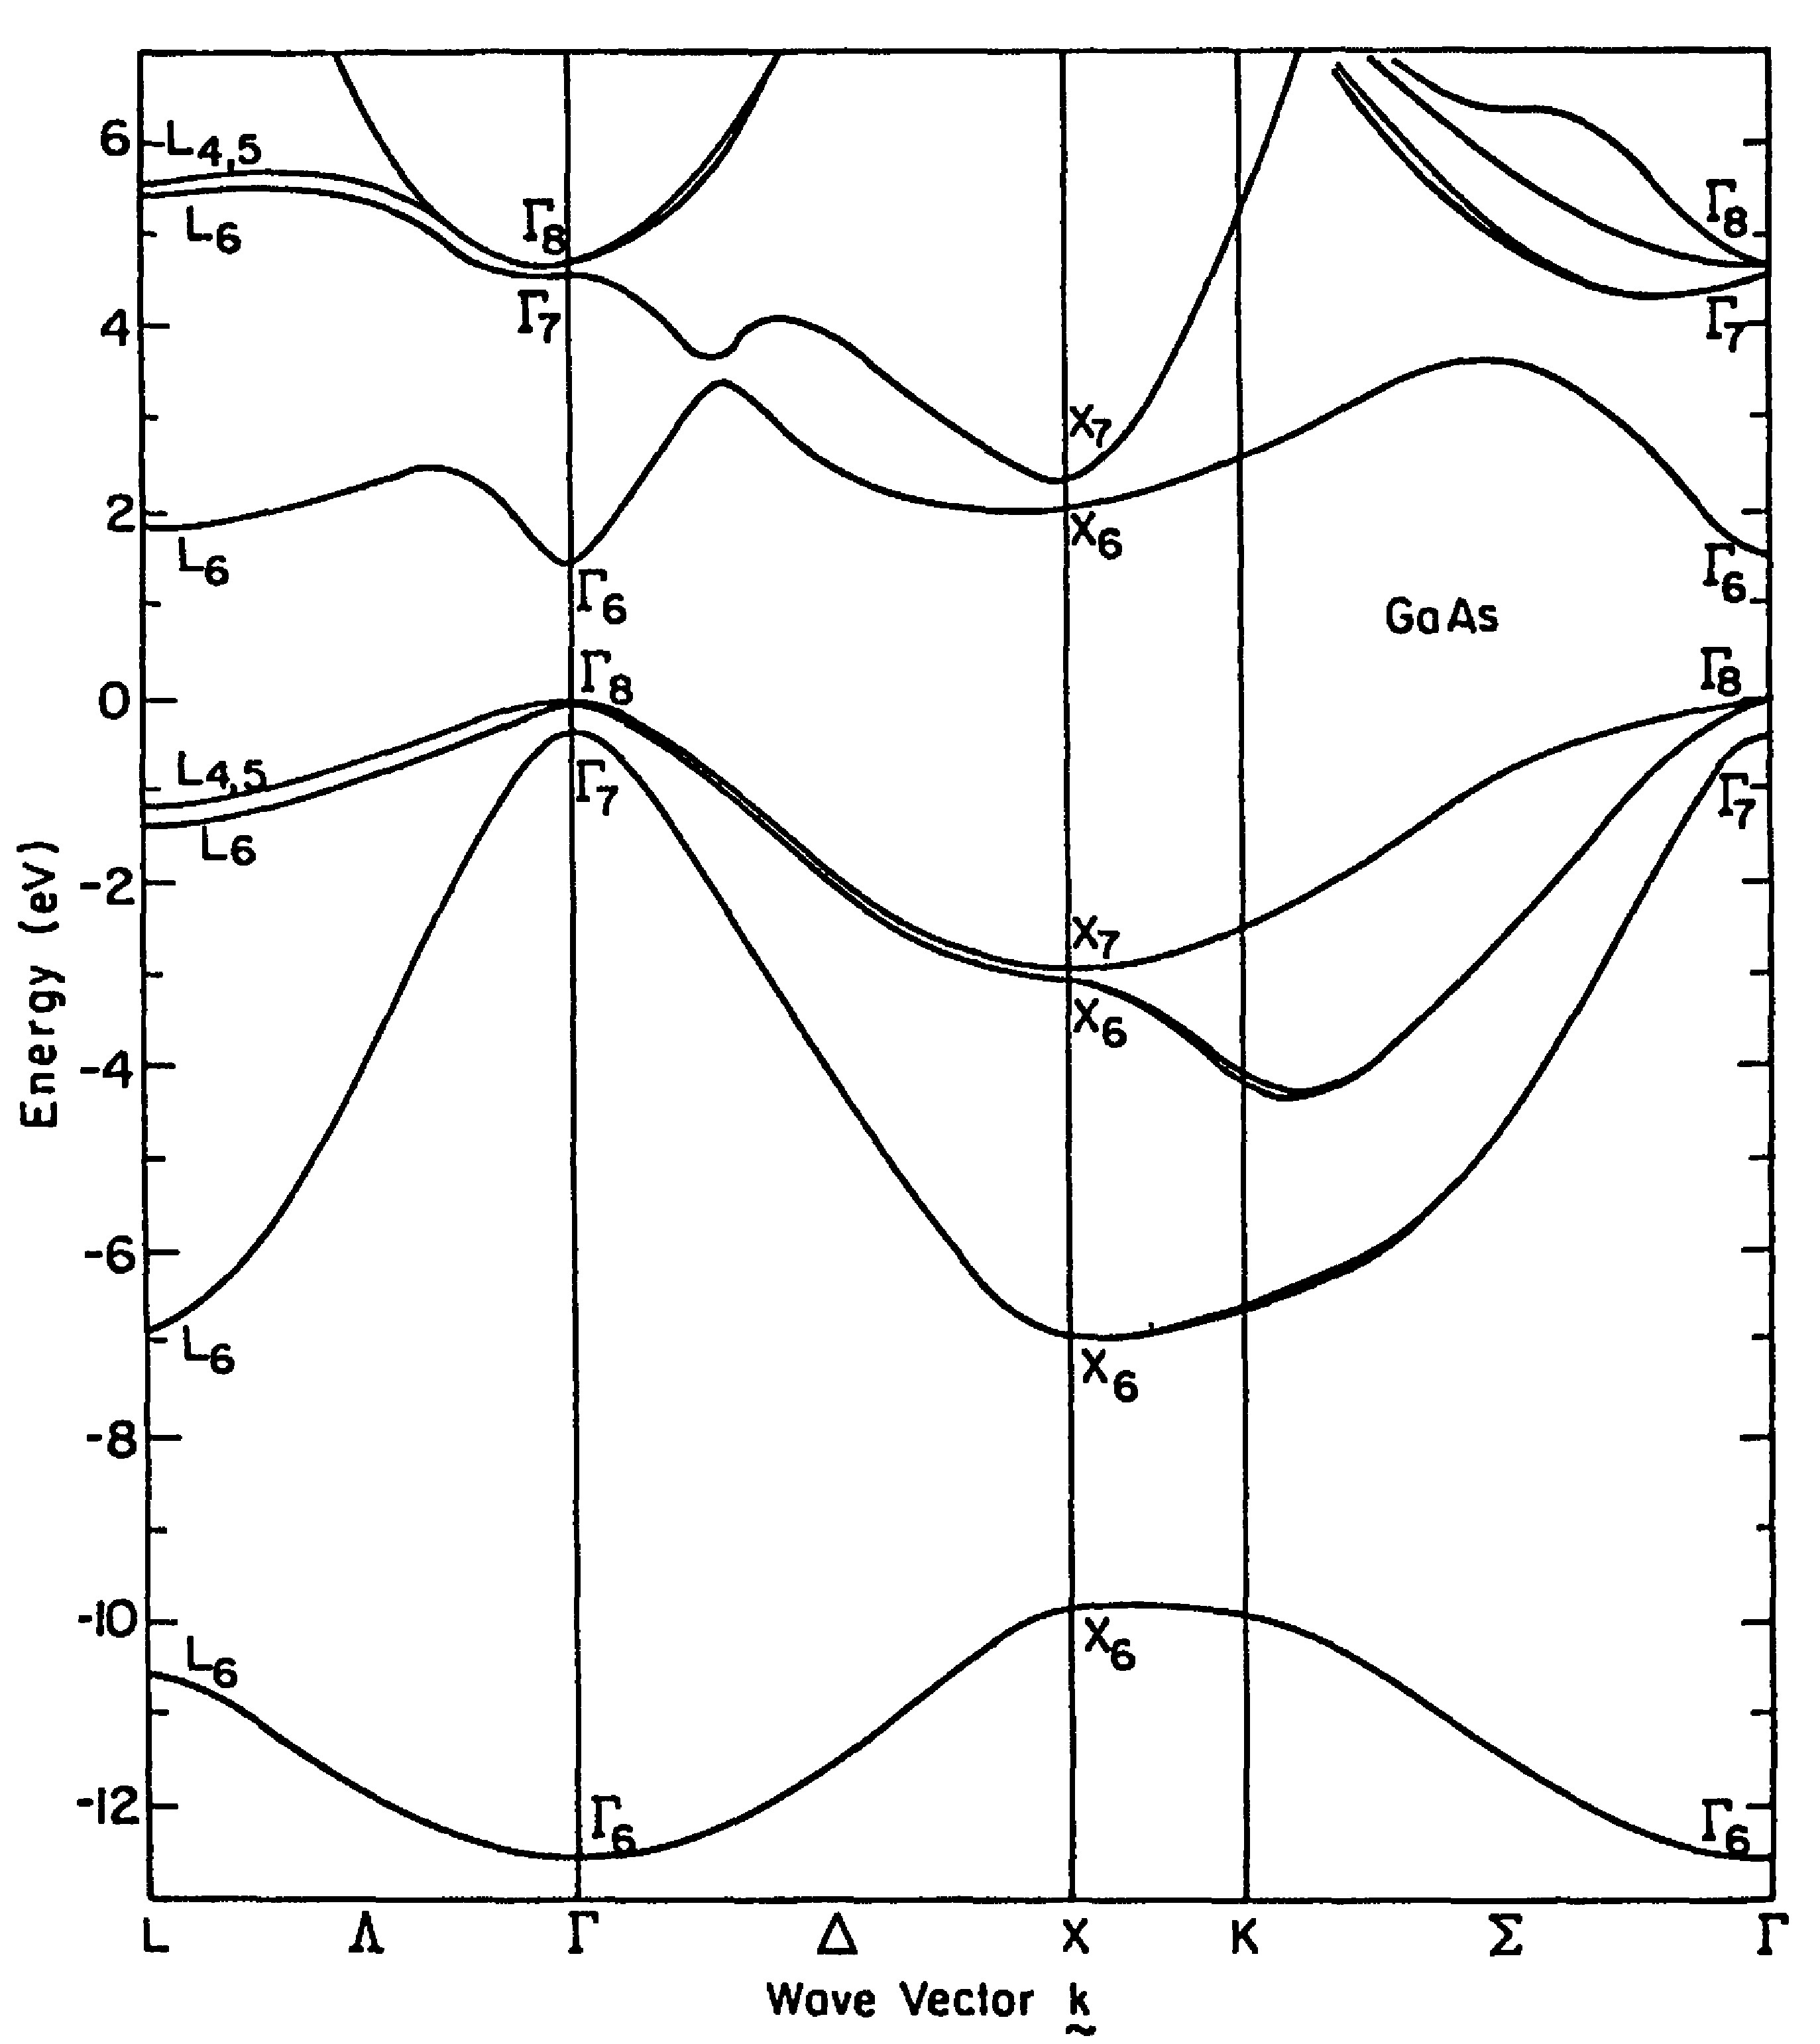
\includegraphics[width=0.6\textwidth]{content/grafik/bandstruktur.jpg}
    \caption{Berechnete Bandstruktur von GaAs um die Bandlücke. \cite{coh_jam_el}}
    \label{fig:band}
\end{figure}

\subsection{Dotierung}

\subsection{Faraday-Effekt}

\begin{figure}
    \centering
    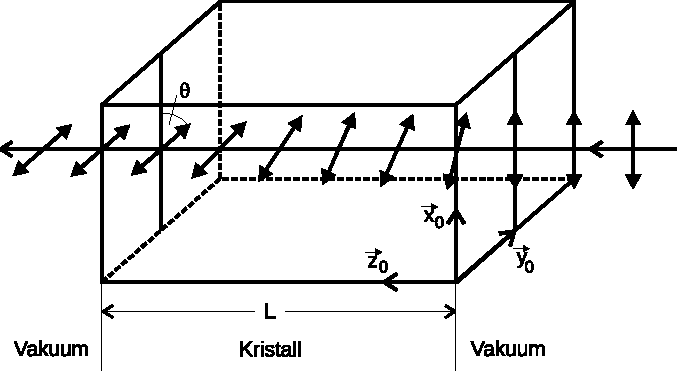
\includegraphics[width=0.7\textwidth]{content/grafik/drehung.pdf}
    \caption{Drehung der Polarisationsebene einer Lichtwelle beim Durchgang durch einen Kristall. \cite{faraday}}
    \label{fig:drehung}
\end{figure}

\begin{align}
    \bm{E}(z) = \pfrac{1}{2} \left(\bm{E}_R(z) + \bm{E}_L(z)\right)
\end{align}

\begin{align}
    \bm{E}_R(z) &= E_0 \left(\bm{\hat{x}} - i \bm{\hat{y}}\right) e^{ik_Rz} \\
    \bm{E}_L(z) &= E_0 \left(\bm{\hat{x}} + i \bm{\hat{y}}\right) e^{ik_Lz}
\end{align}

\begin{align}
    \bm{E}(0) = E_0 \bm{\hat{x}}
\end{align}

\begin{align}
    \bm{E}(L) = \pfrac{1}{2} E_0 \left( 
                \left( e^{ik_RL} + e^{ik_LL} \right) \bm{\hat{x}} +
                \left( e^{ik_RL} - e^{ik_LL} \right) \bm{\hat{y}} \right)
\end{align}

\begin{align}
    \psi &\equiv \pfrac{L}{2} (k_R + k_L) \\
    \theta &\equiv \pfrac{L}{2} (k_R - k_L)
\end{align}

\begin{align}
    \bm{E}(L) = \pfrac{1}{2} E_0 \left( 
                \left( e^{i\psi}e^{i\theta} + e^{i\psi}e^{-i\theta} \right) \bm{\hat{x}} +
                \left( e^{i\psi}e^{i\theta} - e^{i\psi}e^{-i\theta} \right) \bm{\hat{y}} \right)
\end{align}

\begin{align}
    \bm{E}(L) = E_0 e^{i\psi} (\cos\theta \,\bm{\hat{x}} + \sin\theta \,\bm{\hat{y}})
\end{align}
